\documentclass{standalone}
\usepackage{tikz}
\usepackage{amssymb}
\usepackage{fontspec}
\setmainfont{Charis SIL}
\usetikzlibrary{automata, positioning}
\begin{document} 
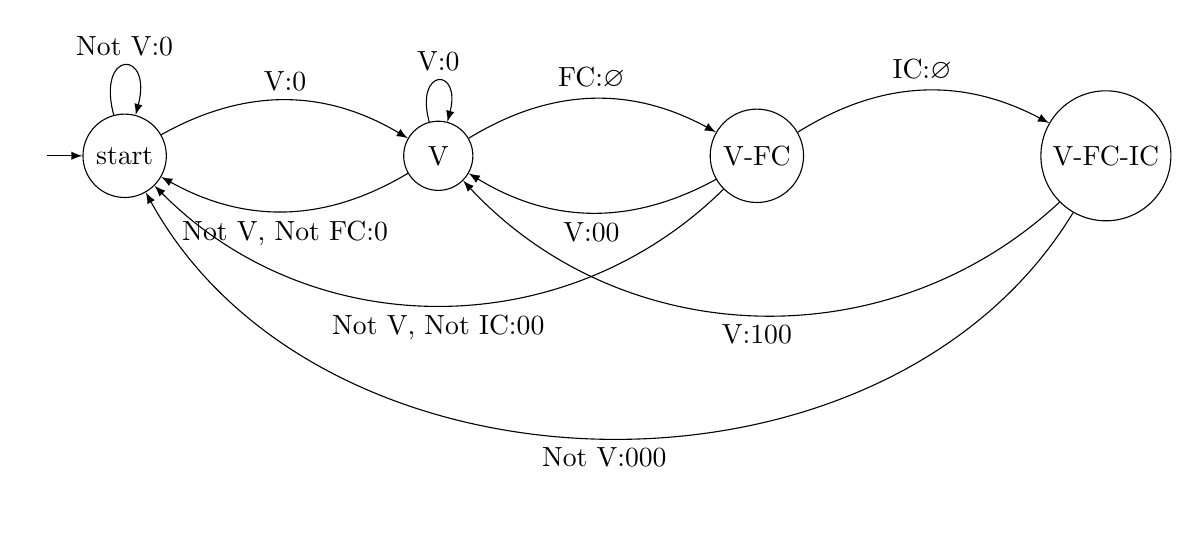
\begin{tikzpicture}[node distance=3cm, auto, every loop/.style={-latex}, every initial by arrow/.style = {-latex}]
\node (q0) [state, initial, initial text = {}] {start};
\node (q1) [state, right = of q0] {V};
\node (q2) [state, right = of q1] {V-FC};
\node (q3) [state, right = of q2] {V-FC-IC};
\path [-latex]
     (q0) edge[bend left] node {V:0} (q1)
     (q1) edge[bend left] node {Not V, Not FC:0} (q0)
     (q1) edge[bend left] node {FC:$\varnothing$} (q2)
     (q2) edge[bend left] node {V:00} (q1)
     (q2) edge[bend left=45] node {Not V, Not IC:00} (q0)
     (q2) edge[bend left] node {IC:$\varnothing$} (q3)
     (q3) edge[bend left=60] node {Not V:000} (q0)
     (q3) edge[bend left=45] node {V:100} (q1)
     (q0) edge[loop above] node {Not V:0}()
     (q1) edge[loop above] node {V:0}();
\end{tikzpicture}
 
\end{document}
